\section{Introduction}
\label{sec:introduction}

Link prediction supports friend recommendation, interaction discovery, and
collaborative filtering. In many deployments, however, the edges needed for
training do not reside in one trusted graph: institutions or clients own
disjoint interaction records and are not allowed to disclose raw
neighborhoods. Federated optimization limits raw-data movement, but it does
not by itself protect an edge from a server that observes model updates or
released representations \cite{mcmahan2017fedavg,dwork2014algorithmic}.
Edge-level differential privacy (DP) supplies a record-level guarantee, but
graph message passing makes both sensitivity and inference subtle. A model
that consults the private graph again when answering a link query can invalidate
an otherwise correct training-time accountant \cite{sajadmanesh2023gap}.

Prior work addresses important portions of this problem. GAP makes private
graph aggregation inference-closed \cite{sajadmanesh2023gap}; DPLP derives
subgraph sensitivity for centralized link prediction
\cite{ran2024dplp}; and decentralized or federated graph learners protect
links, features, representations, or local training processes under several
trust models \cite{lin2022solitude,pei2024lga,li2025pdgl,zhang2025privfgl}.
Private recommendation further shows that edge-DP prediction is meaningful in
heterogeneous and collaborative-filtering settings
\cite{wang2026pphgrl,hu2025cfdpgnn,li2026fedhgpp}. These results make a broad ``first
federated private link prediction'' claim untenable. They also expose a
remaining deployment question:

\begin{quote}
\emph{When a frozen edge-DP structural branch is useful only on some target
graphs, can a federated service activate it without sacrificing either edge
privacy or utility relative to a public-input-only fallback?}
\end{quote}

This question cannot be answered by reporting only the accuracy of a selected
private model. Public descriptors can already be predictive, DP noise scales
with the released structural state, and target graphs differ in how much
additional link signal their private topology contains. In our experiments,
the same frozen structural mechanism produces positive pairwise gains on
BlogCatalog, GitHub Social, PolBlogs, and Deezer, but negative gains on
Facebook and LastFM. A rule that always enables private structure is therefore
not a no-harm policy.

We propose \method{}, illustrated in \cref{fig:overview}. It separates the
\emph{candidate learner} from the \emph{deployment decision}. Any admitted
candidate must release an inference-closed edge-DP state $R$. On a disjoint
set of private certification edges, \method{} computes a bounded
candidate-minus-public pairwise advantage, releases only a Gaussian-noised sum
and count, and activates the candidate when a one-sided lower certificate
exceeds a predeclared material gain $\gamma$. Otherwise it returns the public
branch. All prediction scores are post-processing of public inputs, $R$, and
the private binary decision.

\begin{figure*}[t]
  \centering
  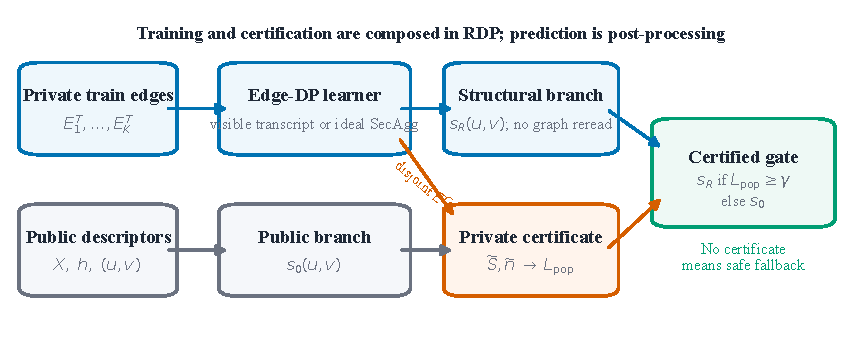
\includegraphics[width=\textwidth]{figures/figure1_certfed_overview.pdf}
  \caption{\method{} separates learning from deployment. The structural
  learner releases an inference-closed edge-DP state from training edges
  $E^T$. A disjoint certification set $E^C$ contributes only a bounded utility
  sum and count. The structural branch is enabled only when the private lower
  certificate reaches $\gamma$; all other cases fall back to the public
  branch. The R5 implementation conservatively composes training and
  certification RDP curves.}
  \label{fig:overview}
\end{figure*}

Our contributions are:

\begin{itemize}
  \item We formulate certified deployment for ordinary-graph federated link
  prediction under add/remove edge adjacency, complete server-transcript
  accounting, cross-client candidates, and inference-closed scoring.
  \item We prove an indistinguishable-worlds result showing that no
  training-only selector has a distribution-free, nontrivial no-harm
  guarantee. Direct target-domain certification is therefore not merely a
  learned dataset selector.
  \item We establish a finite-population no-harm theorem for an edge-keyed
  random certification split. We also derive a sufficient activation boundary
  and a central-DP testing lower bound with matching principal dependence
  $O(\chi/\alpha^2+1/(\eps\alpha))$ up to constants and logarithms.
  \item We conduct a preregistered, one-time, five-seed study on six social and
  blog networks. \method{} safely activates in 15/30 primary cells, avoids all
  ten harmful always-structural cells, and reaches within $0.0057$ mean
  pairwise gain of a non-deployable sign oracle.
\end{itemize}

We do not claim that the registered pairwise certificate is an AUC confidence
interval, that one private learner is universally best, or that ideal secure
aggregation follows from DP. These boundaries are central to the method.
